\section{Safety Factors}\label{appendix-safety}

\newthought{The concept of safety factor has}\marginnote{acknowledgements to Dale O. Anderson, 2001} substantial history behind it. In ancient Rome, the designer of a bridge was required to stand under that bridge after completion while chariots drove over the top. This method of acceptance testing put the bridge designer's life at risk as well as the lives of those who used the bridge. The idea was obviously to induce the bridge designer to design and build a safe bridge. Safe designs were then copied.

The desire for safe structures and machines is the same today as it was anciently. Modern engineering is based on predicting the performance of structures and machines before they are actually built. This requires an assessment of how well the system performance can be predicted for the intended materials, expected use, foreseeable abuse, the expected service environment, and the expected life of the system. The transition from engineering model to reality is usually facilitated by including a factor of safety in the design to accommodate uncertainty in material properties and the design process, the consequences of failure, risk to people, and degree of characterization of and control over the service environment. The safety factor for structural systems, proposed Philon of Byzantium (3rd century BC)~\cite{joseph2001}, is defined as follows:

\begin{equation}
  N = \frac{\text{capacity}}{\text{load}} = \frac{\text{strength}}{stress} > 1
  \label{equ-safety-1}
\end{equation}

Notice that safety factor is a simple ratio that is intended to be greater than one. That is, capacity must be greater than load and strength must be greater than stress. A large safety factor usually means a safer design, however, more material is used in the design with a corresponding increase in cost and weight. Therein lies one of the fundamental trade-offs in engineering design – cost vs. safety. Reducing cost is always a business imperative, while the public demands increased safety. Professional organizations frequently specify minimum safety factors for various systems. It is incumbent on the design engineer to choose an adequate safety factor to safeguard public safety at an affordable cost.

Aerospace systems require minimal weight structures, thus demanding low safety factors. Aerospace systems also undergo extensive physical testing of materials, components, and structures to validate the design before production, which is a very costly and time consuming process. A military missile, for example, may have a safety factor of 1 because it is intended for use only once and has a relatively short life. A fighter aircraft may have a safety factor as low as 1.2, but the air crews have ejection seats and parachutes and the airframe undergoes regular inspection and maintenance. A commercial aircraft may have a safety factor as low as 1.5, but it also is inspected and maintained regularly. On the other end of the spectrum, a concrete dam may have a safety factor as high as 20 because the expected life is several decades and it is a brittle structure for which failure would be catastrophic.

The load bearing capacity or strength of a material is determined by physical testing. The properties of a specific material are random variables that are assumed to follow a normal distribution with a mean value and a standard deviation. A material varies in composition from factory to factory and from batch to batch in production, with a corresponding variation in properties. Material properties also vary according to the processing applied to the material to shape and strengthen it as desired. In some materials, properties may vary significantly over time. Corrosive service environments may attack the surface of the material and cause corrosion, erosion, and/or cracking over time, thus reducing material strength. High temperature service environments usually reduce material strength significantly. Cyclic loading of a material can lead to a fatigue failure over time. Impact (shock) loading produces very high transient stresses which can precipitate failure.

The load and stress values for the structure usually come from an engineering model and depend on system geometry, intended use, foreseeable abuse, service environment, anticipated material deterioration over time, etc. The load on a member in the structure is based on the external loads applied to the whole structure, the reactions supporting the structure, and the geometry of the structure. Variations in external loads, reactions, and/or geometry result in variations of calculated load. Thus load, and therefore stress, is also a random variable with an expected mean value and a standard deviation.

\subsection{Reliability}

Equation~\ref{equ-safety-1} is called the central safety factor if it is based on mean values of capacity, strength, load, and stress. This means, for example, that approximately 50\% of the parts made out of a particular material will have a strength less than the mean value, and the rest will have a strength greater than or equal to the mean value. If one were to design a part for mass production using the mean strength value, approximately half of the parts produced would be of lower strength than desired. This might pose a problem over the service life of those systems. Suppose the loading on the system were actually greater than anticipated in the design and the strength of the system were less than expected, then the probability of failure of that system would be greater than expected. \cref{fig-prob-dist} depicts normal probability distributions of both stress and strength which overlap. The region of overlap is also the region of greatest probability of system failure.

\begin{figure}
  \centering
  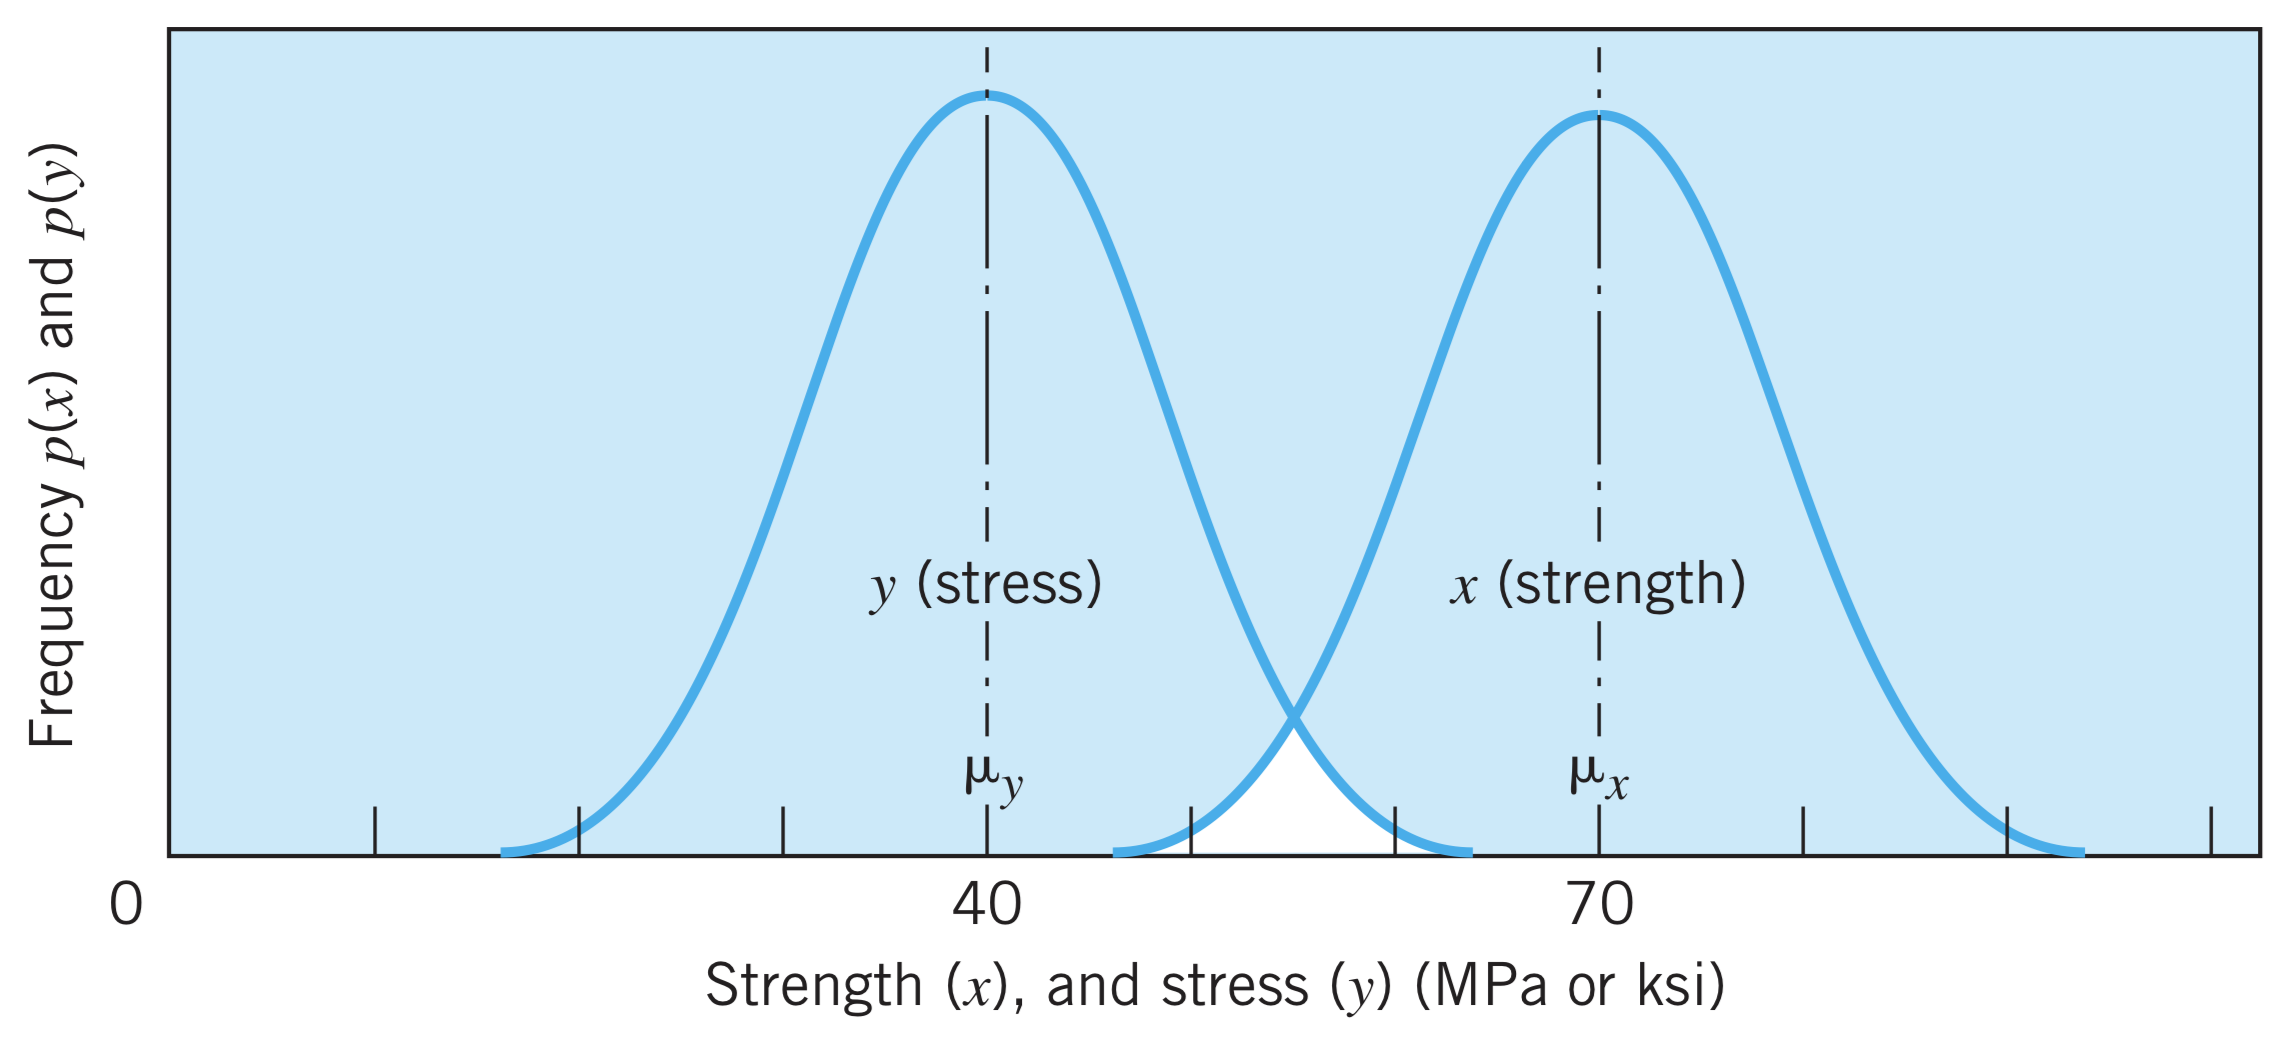
\includegraphics[width=0.9\textwidth]{figs/stress-strength-dist.png}
  \caption[The probability distributions of stress and strength showing substantial overlap]{The probability distributions of stress and strength showing substantial overlap~\citep{juvinall1983}}
  \label{fig-prob-dist}
\end{figure}

Based on \cref{fig-prob-dist}, we may modify the safety factor Equation~\ref{equ-safety-1} to account for this overlap between stress and strength as follows~\cite{joseph2001}:

\begin{equation}
  N_R = N \bigg( \frac{1-a\gamma_s}{1+a\gamma_\sigma} \bigg) > 1
  \label{equ-safety-2}
\end{equation}

\noindent where:

\begin{description}
  \item[$N_R$] is the safety factor based on reliability
  \item[$N$] is the central safety factor based on mean or expected values (Equation~\ref{equ-safety-1})
  \item[$\gamma_s$] is the coefficient of variation of the strength value (published or estimated)
  \item[$\gamma_\sigma$] is the coefficient of variation of the stress value (estimated)
  \item[$a$] is the number of standard deviations to produce the desired confidence level (Table~\ref{tbl-a})
\end{description}

\begin{table*}
  \center{}
  \small
  \begin{tabular}{l r r r r r r r r}
    \toprule
    $a$ & 0 & 1.65 & 2.33 & 3 & 3.08 & 3.62 & 4.42 & 4.89 \\
    \midrule
    Reliability & 50\% & 95\% & 99\% & 99.87\% & 99.9\% & 99.99\% & 99.999\% & 99.9999\% \\
    Failure Rate & $\frac{1}{2}$ & $\frac{1}{20}$ & $\frac{1}{100}$ & $\frac{1}{769}$ & $\frac{1}{1000}$ & $\frac{1}{10000}$ & $\frac{1}{100000}$ & $\frac{1}{1000000}$ \\
    \bottomrule
  \end{tabular}
  \vspace{2em}
  \caption{Values for $a$}
  \label{tbl-a}
\end{table*}

Notice that Equation~\ref{equ-safety-2} is a relatively simple modification of the definition of central safety factor (Equation~\ref{equ-safety-1}) that compares the highest expected stress against the lowest expected strength based on the specified level of reliability.

\begin{figure}
  \centering
  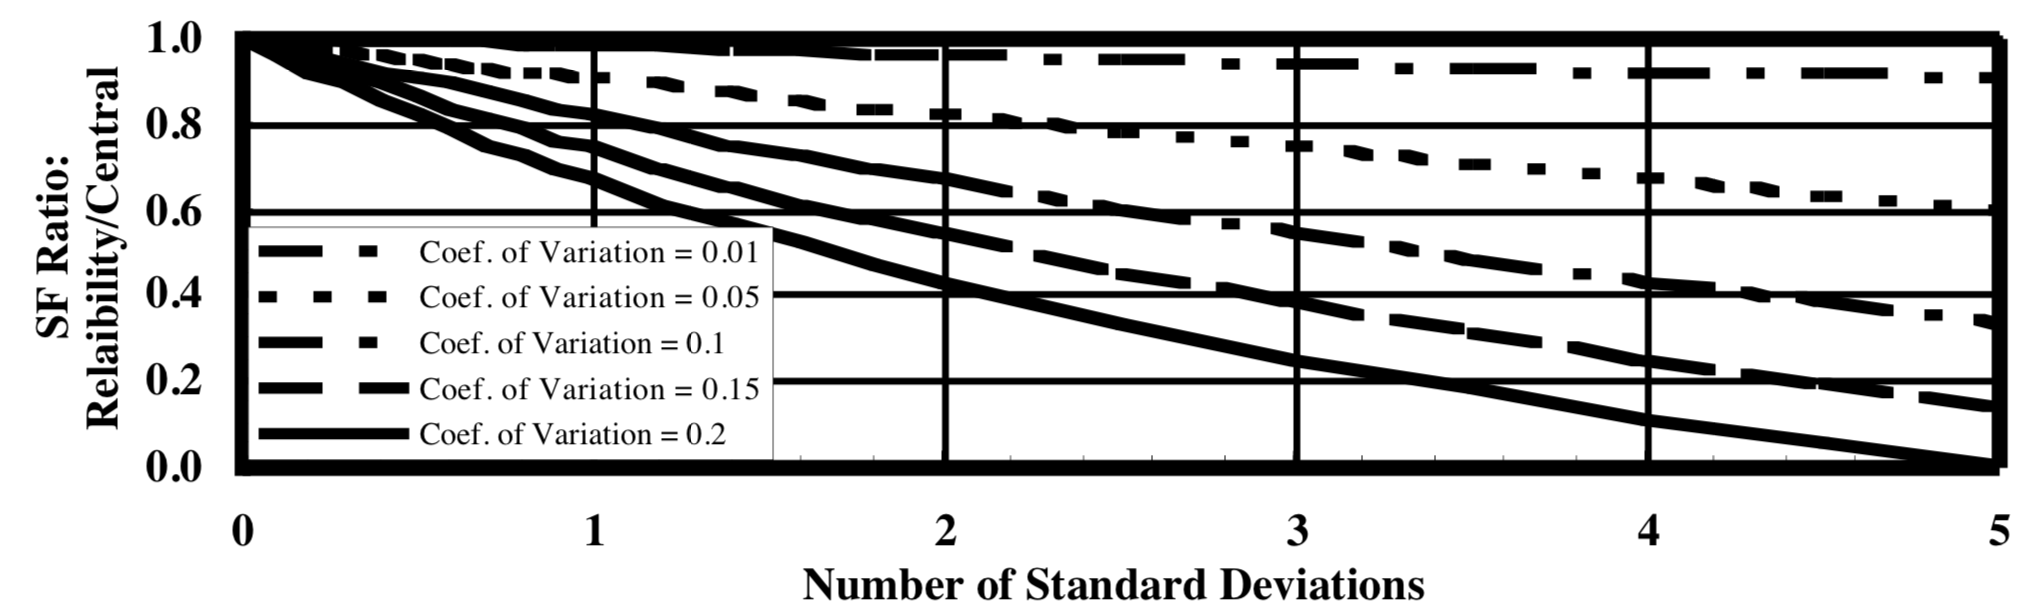
\includegraphics[width=\textwidth]{figs/sf-ratio.png}
  \caption{Ratio of the reliability safety factor to the central safety factor}
\end{figure}

\subsection{The Visodic Safety Factor Model}

Joseph P. Visodic developed and published recommendations for minimum central safety factor values in 1948 which were based on cumulative experience~\cite{joseph2001}\cite{juvinall1983}. These are presented in Table~\ref{tbl-visodic}. Safety factors for ductile materials are based on yield strength. Safety factors for brittle materials are based on ultimate strength and are twice the recommended values for ductile materials. Safety factors for primarily cyclic loading are based on endurance limit. Impact loads require a safety factor of at least 2 multiplied by an ``impact factor'', usually in the range of 1.1 to 2.

\begin{table}
    \footnotesize
    \centering
    \begin{tabular}{p{0.15\textwidth} p{0.15\textwidth} p{0.15\textwidth} p{0.15\textwidth} p{0.15\textwidth}}
      \toprule
        Safety Factor & Knowledge of Loads & Knowledge of Stress & Knowledge of Material & Knowledge of Environment \\
      \midrule
        1.2-1.5 & Accurate & Accurate & Well Known & Controllable \\
        1.5-2.0 & Good & Good & Well Known & Constant \\
        2.0-2.5 & Good & Good & Average & Ordinary \\
        2.5-3.0 & Average & Average & Less Tried & Ordinary \\
        3.0-4.0 & Average & Average & Untried & Ordinary \\
        3.0-4.0 & Uncertain & Uncertain & Better Known & Uncertain \\
      \bottomrule
    \end{tabular}
  \caption[Recommended central safety factors for ductile materials based on yield strength]{Recommended central safety factors for ductile materials based on yield strength~\citep{joseph2001}}
  \label{tbl-visodic}
\end{table}

\subsection{The Norton Safety Factor Model}

Robert L. Norton~\cite{robert2006} stated ``Clearly, where human safety is involved, high values of (safety factor) are justified''. His overall safety factor value is a combination of a safety factor based on material properties, one based on engineering model accuracy, and one based on expected service environment, as follows:

\begin{eqnarray}
  N_{\text{ductile}} \geq \max(N_1, N_2, N_3); \text{ based on yield strength} \\
  N_{\text{brittle}} \geq 2\times\max(N_1, N_2, N_3); \text{ based on ultimate strength}
\end{eqnarray}

\noindent Where $N_1, N_2$ and $N_3$ are selected from Table~\ref{tbl-norton}.

\begin{table}
  \centering
  \small
  \begin{tabular}{p{0.1\textwidth} p{0.25\textwidth} p{0.25\textwidth} p{0.25\textwidth}}
    \toprule
      Safety Factor & $N_1$ & $N_2$ & $N_3$ \\
      & Material Properties (from tests) & Stress/Load Model Accuracy & Service Environment \\
    \midrule
    1.3 & Well known/characterized & Confirmed by testing & Same as material test conditions \\
    2 & Good approximation & Good approximation & Controlled, room-temperature \\
    3 & Fair approximation & Fair approximation & Moderately challenging \\
    5+ & Crude approximation & Crude approximation & Extremely challenging\\
    \bottomrule
  \end{tabular}
  \label{tbl-norton}
  \caption[Recommended central safety factors for ductile materials based on yield strength]{Recommended central safety factors for ductile materials based on yield strength~\citep{robert2006}}
\end{table}

\subsection{The Pugsley Safety Factor Model}

Please see \cref{sec:DF}.

\subsection{Misc. Safety Factor Models}

Lipson and Juvinall~\cite{lipson1963} presented the safety factor recommendation shown in tables 4 and 5, which were based on cumulative experience. In order to compare the values in these tables with the values in the previous tables, let us assume that the yield strength of hot rolled steel is half of the ultimate strength, therefore the safety factors can be cut in half (except for those listed for cast iron, which is brittle).

\begin{table}
  \centering
  \small
  \begin{tabular}{p{0.3\textwidth} c c}
    \toprule
    Kind of Load & Steel (Ductile) & Cast Iron (Brittle) \\
    \midrule
    Dead (static) load & 5 & 6 \\
    Repeated, gradually applied in one direction with mild shock & 6 & 10 \\
    Repeated, gradually applied in reversed directions with mild shock & 8 & 15 \\
    Shock load & 12 & 20 \\
    \bottomrule
  \end{tabular}
  \caption{recommended safety factors based on ultimate strength}
\end{table}

\subsection{Discussion and Recommendations}

The value of a central safety factor (Equation~\ref{equ-safety-1}) should not be less than two (2) for most structural applications and should routinely be set at three (3). Low safety factors are justified only where extensive physical testing of both materials and structural systems is done. Low safety factors also require routine periodic inspection and maintenance of the system if it is to have a useable life of more than a few years in an ordinary service environment. Uncertainty in loading, uncertainty in material properties, foreseeable abuse, and challenging service environments demand higher values of the safety factor. A long service life also requires a larger value of safety factor. High reliability applications require systems with a larger central safety factor value.

The reliability safety factor (Equation~\ref{equ-safety-2}) accommodates lower values than the central safety factor (Equation~\ref{equ-safety-1}) for the same probability of failure. Shigley~\cite{joseph2001} feels that given well known values and a reasonable reliability level (95\% or higher) safety factor values between 1.3 and 2.0 are adequate. Again, lower safety factor values require physical testing, a predictable service environment, and periodic inspection and maintenance.

Brittle\marginnote{Brittle Materials} materials require a higher safety factor than ductile materials because brittle failure is abrupt and not preceded by yielding. The consensus in the literature is that the safety factor for brittle materials should be at least twice that used for ductile materials and should be based on ultimate strength.

Service\marginnote{Service Loads} loads due to expected normal use and foreseeable abuse are usually difficult to establish. Well characterized loads justify a lower minimum safety factor value, while uncertain loads require a larger value.

Cyclic loading\marginnote{Cyclic Loading} induces fatigue failure in structural components. The safety factor for primarily cyclic loading should be based on the endurance limit rather than on yield or tensile strength. Well characterized cyclic loads justify a lower minimum safety factor value, while uncertain loads should have a larger value.

Impact\marginnote{Impact Loading} (shock) loading induces very high transient stresses in structural components that can precipitate failure. Therefore the safety factor for impact loading should be at least 2.0, and 1.5 to 2.5 times that used for static (dead) loads. The greater the impact force, the higher the safety factor needed.

The consequences of system failure must also be considered in the selection of a minimum safety factor value. If human life and health are not at risk and potential property damage is limited to the system itself, then the minimum safety factor value may be lowered a little. However if human life and health are at risk and/or potential property damage caused by system failure is substantial, then a higher minimum safety factor value is required. These are the situations in which failure precipitates liability litigation and therefore a higher safety factor should be viewed as relatively cheap liability insurance.

The service life of the system is important in the selection of a minimum safety factor value. A short expected service life justifies a lower minimum safety factor value, while a long expected service life demands a higher value.

The service environment also affects the selection of a minimum safety factor value. A controlled indoor environment may accommodate a lower minimum safety factor value, while a challenging environment involving temperature extremes, corrosion, earthquake, occasional high winds, etc. needs a substantially larger value.

\begin{table}
    \centering
    \small
    \begin{tabular}{p{0.5\textwidth} c c c}
      \toprule
        Test Case & Visodic & Norton & Pugsley \\
      \midrule
        \textbf{Commercial aerospace structure:} Very well tested materials and structures. Well Characterized loads. Predictable service environment. Periodic inspection and maintenance throughout long life. Failure usually results in high risk to many human lives. (A SF of 1.5 is expected.)
        & 1.2-1.5
        & 1.3
        & 1.4
        \\
        \textbf{Trailer hitch coupler:} Defined maximum loads by class. Occasional service loads 2-3 times defined maximums. Corrosive environment. Cyclic and impact loading. Very little inspection and maintenance during moderately long life. Failure may result in high risk to human life.
        & 4.0-6.0
        & 4.0
        & 4.0
        \\
        \textbf{Large utility power transformer:} Well defined maximum loads. Occasional service loads 1-2 times normal. Cyclic and impact loading. Predictable but challenging service environment. Periodic inspection and maintenance throughout very long life. (A SF of 5 is customary.)
        & 3.8-5.0
        & 4.0
        & 3.8
        \\
      \bottomrule
    \end{tabular}
  \caption{a comparison of safety factor models}
\end{table}
